\documentclass{article}
\usepackage{graphicx}
\usepackage[T1]{fontenc}
\usepackage[utf8]{inputenc}
\usepackage{hyperref}
\usepackage{geometry}
\usepackage{mwe}
\usepackage[hungarian]{babel}
\usepackage{upquote}              % for proper verbatim characters

\textwidth=450pt
\begin{document}

\title{ELTE Haladó labor, Piszkéstető}
\author{Szakáts Róbert, Sódor Ádám}

\maketitle
\tableofcontents
\newpage

\section{Előfeltételek}
\begin{itemize}
  \item Saját otthoni gépen futó, modern linux operációs rendszer, pl. Debian 10.
  \item bash (\url{http://www.tldp.org/LDP/Bash-Beginners-Guide/html/})
  \item FITSH (\url{https://fitsh.net/})
  \item Gnuplot (\url{http://www.gnuplot.info/})
  \item awk (\url{https://www.linuxtechi.com/awk-command-tutorial-with-examples/})
  \item ds9 (\url{http://ds9.si.edu/site/Home.html})
  \item xpatools (\url{http://hea-www.harvard.edu/saord/xpa/})
\end{itemize}

A labor során piszkéstetői archív méréseket fogunk feldolgozni. A méréseket,
illetve a laborhoz szükséges szkripteket, fájlokat a labor honlapjáról lehet
letölteni:
\url{https://konkoly.hu/staff/szakats.robert/}

A felsorolt szoftvereket próbáljuk meg még a labor előtt feltelepíteni.
Egy részük (bash, awk, gnuplot) sok esetben már az alaprendszerrel feltelepül.
A {\bf{FITSH}} telepítése a honlapján elég jól le van írva, illetve bizonyos
disztribúciókban (pl. Debian) elérhető repóból is, mint ahogy a ds9 is.

A szoftverek telepítése után töltsük le az adatfájlokat és az egyéb fájlokat a
gépünkre egy munkakönyvtárba. Kb. 10GB szabad helyre lesz majd szükség.
Tömörítsük ki a data.tar.bz2 fájlt:
\begin{verbatim}
  tar -xvf data.tar.bz2
\end{verbatim}


Az {\it imexam} és a {\it tvmark} szkripteket másoljuk át a \$HOME/bin/ mappába
és tegyük végrehajthatóvá:
\begin{verbatim}
  chmod +x imexam
\end{verbatim}


Ha még nem lenne benne a \$HOME/.bashrc-ben a következő sor, akkor írjuk bele:
\begin{verbatim}
  export PATH="$PATH:$HOME/bin/"
\end{verbatim}

\section{Bevezetés}

A labor során egy pulzáló változócsillagról (XX Cyg) készült méréseket fogjuk
feldolgozni. A mérések a piszkéstetői Schmidt távcsővel készültek.

Linuxos környezetben fogunk dolgozni, így az alapvető linuxos parancsok és
valamilyen ismertebb linux alapszintű felhasználói ismerete előny.

A feldolgozás során elvégezzük az alapvető képkorrekciókat, úgy mint bias, dark
és flat, majd megcsináljuk a fotometriát (fényességmérés) és végül ábrázoljuk a
csillag fénygörbéjét, azaz a (jelen esetben relatív) fényességváltozását az idő
függvényében.
Végül pedig házi feladat keretében a jegyzőkönyvnek kell elkészülnie.

Az alapvető képkorrekciókról és a CCD kamerák működéséről a feltöltött
{\it ccd.pdf}-ből készüljünk fel.

Az apertúra fotometriához jó bevezető a következő dokumentum:
\url{http://web.ipac.caltech.edu/staff/fmasci/home/astro_refs/aperture_phot2.pdf}

A többi használt szoftverhez az előző fejezetben található linkeken lehet
információt szerezni.

A következő feladatok során a parancsok kiadása minden esetben linux
parancssorban történik, kivéve ott, ahol ez jelezve van.

\section{Fits fájlok kezelése}

Ebben a feladatban megismerkedünk a fits fájlformátummal és hogy hogyan tudunk
ezekből a fájlokból információt kinyerni, illetve hogyan tudjuk megjeleníteni.

Maga a formátum a Flexible Image Transport System rövidítése. Ez egy standard,
digitális formátum, amelyben adatokat tudunk tárolni. Ez lehet kép információ
is, de táblázat is. Akár több dimenziós, úgynevezett datacube-ok is lehetnek
fits fájlokban.

A mi esetünben az összes fájl egy-egy csillagászati felvétel, vagy ahhoz
kapcsolódó kalibrációs kép.
Minden fájlunk két részből áll: egy header, vagy fejlécből és magából az
adatból. A fejlécben mindenféle hasznos információk és kommentek találhatók,
amihez többféleképpen is hozzáférhetünk.
A FITSH csomag fiheader task-ja tudja olvasni és írni a header részt.
Pl.:

\begin{verbatim}
  fiheader bias_1x1_0001_bias.fits --get date-obs
\end{verbatim}

melynek kimenete:
\begin{verbatim}
  2018-10-13T04:18:17.8266
\end{verbatim}

Ez az adott felvétel készítési ideje, UT-ban, ISOT formátumban.
Ebben a példában a date-obs egy fejléc keyword, vagy kulcsszó volt, a --get
pedig az, hogy olvasni akarjuk az adott kulcsszó értékét.

A --set paranccsal írni is tudunk a fejlécbe, pl.:
\begin{verbatim}
  fiheader bias_1x1_0001_bias.fits --set teszt='Teszt proba'
\end{verbatim}

Majd nézzük meg, hogy sikerült-e:
\begin{verbatim}
  fiheader bias_1x1_0001_bias.fits --get teszt
\end{verbatim}

{\bf Feladat:}
A következő fájlokból olvassuk ki az alább felsorolt kulcsszavak értékét és
jegyezzük fel:
Fájlok:
\begin{itemize}
  \item bias\_1x1\_0001\_bias.fits
  \item dark-30sec\_1x1\_0001\_dark.fits
  \item domeflatr\_0001\_R.fits
  \item XX\_Cyg-20181012\_0001\_R.fits
\end{itemize}
Kulcsszavak:
\begin{itemize}
  \item date-obs
  \item imagetyp
  \item filter
  \item ccdtemp
\end{itemize}


A képek megjelenítéséhez a ds9 nevű programot fogjuk használni.
Nyissunk meg egy objektumképet a ds9-ben. Írjuk pe a parancssorba:
\begin{verbatim}
  ds9 XX_Cyg-20181012_0001_R.fits -scale zscale&
\end{verbatim}

\begin{figure}
    \centering
    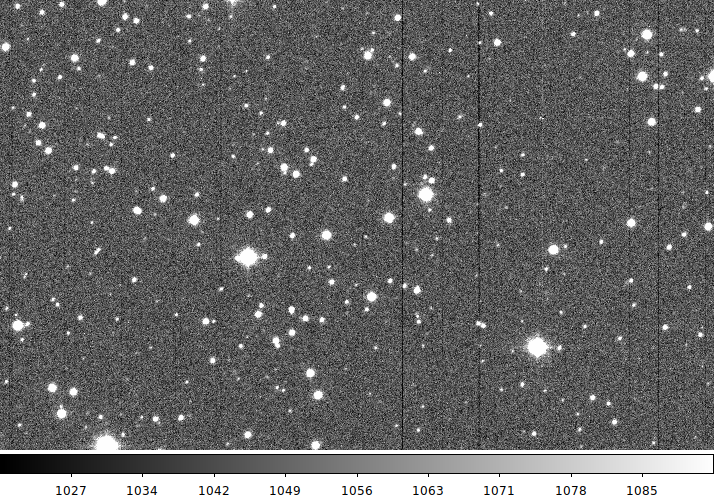
\includegraphics[width=0.8\linewidth]{pics/object.png}
    \caption{Megnyitott objektumkép a ds9-ben.}
    \label{objds9}
\end{figure}

Láthatjuk, hogy a képen rengeteg csillag található. A zoom menüben zoomolhatunk,
vagy az egérgörgővel is. A felvételek a Schmidt távcsővel készültek, aminek a
látómezeje az égen majdnem 1.1x1.1 fok. Összehasonlításképpen, a telihold fél
fok átmérőjű.
A képen látszanak még hibás pixel oszlopok, amik a kamera elöregedése miatt
jelentek meg. Ezeknek a nagy részét remélhetőleg a bias és dark korrekció
kiszedi majd.
Ha már fut a ds9, akkor a File menüben megnyithatunk másik fits fájlt is.

{\bf Feladat:}
Hasonlítsuk össze a bias, dark, flat és objektumképeket.
A ds9 Frame menüjében nyithatunk új frame-et. Ezek mindegyikáben egy-egy külön
fits fájlt tudunk megjeleníteni. Váltani köztük a TAB gomb lenyomásával tudunk.
Nyissuk meg külön framekben az előző feladatban szereplő fájlokat. Írjuk le a
szemmel végzett összehasonlítások tapasztalatait. Csináljunk képeket a
jegyzőkönyvbe:
File - Save image - PNG...

A ds9 nem csak a kép adatrészét tudja megjeleníteni, de a fejlécet is. Ezt a
File - Header gomb megnyomásával tudjuk megtenni. Egy új ablakban megjelenik a
teljes fejléc. Ellenőrizzük az előző feladatban kinyert kulcsszavak értékét.

Tipp: A képeket egymás mellett is meg tudjuk jeleníteni. Ekkor a Frame - Tile
gombot kell megnyomi, majd Frame - New és File - Open.

\section{Redukálás}

Mint láttuk, a nyers csillagászati felvételek nem alkalmasak tudományos mérések
elvégzésére. Ehhez először az alapvető képredukciós lépéseket kell megtennünk,
azaz a bias, dark és flat korrekciót.
Nagyon fontos, hogy az eredeti fájlokat ne írjuk felül!
Ehhez hozzuk létre az alábbi alkönyvtárakat a munkakönyvtárunkban:
\begin{itemize}
  \item master
  \item reduced
\end{itemize}
Tipp: használjuk az mkdir parancsot.

\subsection{Master bias}
Először a master, azaz átlagolt bias képet készítjük el. Ehhez a FITSH ficalib
és ficombine taskjait fogjuk használni.

Először a szaturációra és a gain-re korrigáljuk a fájlokat. A FITSH taskjai sok
esetben elfogadnak listákat, így mi is azt fogunk használni most, egy bash
változó képében.

A fájlokat a fejlécek alapján fogjuk szétválogatni. Sajnos a gyakorlati
tapasztalat azt mutatja, hogy a fájlnevek nem mindig utalnak a mérés típusára.
A mi esetünkben ez nem így van szerencsére, de mindenesetre most a biztosabb
megoldást fogjuk használni.

Adjuk ki a következő parancsot ott, ahol a fájljaink vannak:
\begin{verbatim}
  fiheader *.fits --get imagetyp | awk '$2=="bias"{print $1}'
\end{verbatim}

Itt az awk-ot használtuk arra, hogy egy adott feltételre leszűrjük a
fájlneveket. A $|$ jel a pipe, ezzel tudjuk az egyik parancs kimenetét egy
másik bemenetére irányítani.
{\bf Feladat:}
Futassuk le a fenti parancsot a pipe és az awk nélkül. Látjuk, hogy a második
oszlop az imagetyp kulcsszó értéke, míg az első a fájlnév. Az awk a \$1, \$2,
stb. módon hivatkozik az oszlopok sorszámára. A számozás egytől indul. A \$0 a
teljes sort kiíratja.

Ez simán a konzolba írja ki a fájlokat, de nekünk most jobb lenne egy
változóban eltárolni őket.

Bash változónak a következő módon adhatunk értéket:
\begin{verbatim}
  biaslist=$(fiheader *.fits --get imagetyp |\
  awk '$2=="bias"{print $1}')
\end{verbatim}

Írassuk ki a változó értékét:
\begin{verbatim}
  echo $biaslist
\end{verbatim}

Látjuk, hogy a bias fájljaink nevei vannak benne. Ezzel már tudunk tovább
dolgozni.
Mivel nem akarjuk felülírni az eredeti fájljainkat, hozzunk létre az ideiglenes
fájloknak is egy listát. Ezeket nyugodtan létrehozhatjuk a /tmp mappában,
ahonnan később törlésre kerülnek majd.
Egyesével macerás lenne ezt megcsinálni, ezért a bash-ben lévő for ciklust
fogjuk használni:

\begin{verbatim}
  for j in $biaslist;do echo "/tmp/r"$j;done
\end{verbatim}

{\bf Feladat:}
Ez még csak kiírta az ideiglenes fájlok nevét. Az előző példa alapján rakjuk
ezeket is egy bash változóba, aminek a neve legyen rbiaslist.

Ha ez kész, végezzük el a szaturáció és gain korrekciót:
\begin{verbatim}
  ficalib -i $biaslist --saturation 46000 --gain 1.7 \
  -o $rbiaslist
\end{verbatim}

Itt a ficalib taskot használjuk, ami bemenetnek a nyers bias fájlkat kapja meg,
elvégzi a korrekciókat, majd kiírja a korrigált fájlokat.

Majd létrehozzuk a master bias képet:
\begin{verbatim}
  ficombine $rbiaslist --mode median -o master/BIAS.fits
\end{verbatim}

\begin{figure*}[ht!]
    \centering
    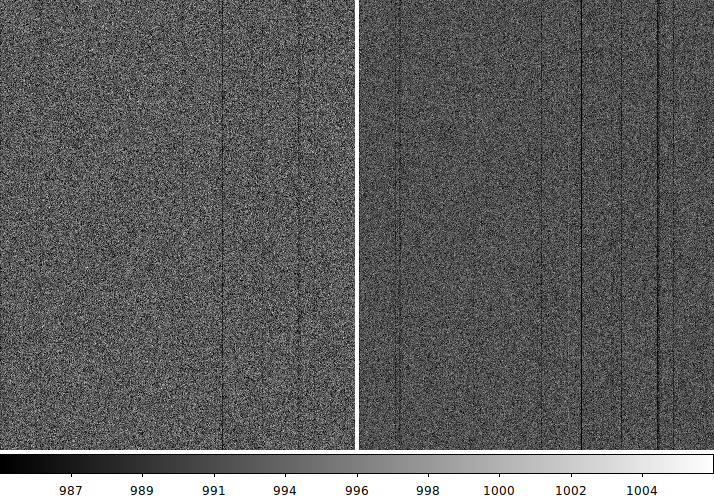
\includegraphics[width=0.8\linewidth]{pics/biascomp.png}
    \caption{Nyers bias kép és a master bias összehasonlítása.}
    \label{biascomp}
\end{figure*}

Itt az előző lépésben korrigál fájlokból létrehozza az átlagolt master bias
képet. Bias és dark képeknél a sima átlag is jó, de flatnél mindenképpen medián
átlagot vegyünk.

Kitörölhetjük az ideiglenes fájlokat:
\begin{verbatim}
  rm /tmp/r*.fits
\end{verbatim}

{\bf Feladat:}
Nyissuk meg ds9-ben a master bias-t és egy másik frame-ben egy sima bias képet.
Hasonlítsuk őket össze. Tapasztalatainkat írjuk le a jegyzőkönyvbe.


\subsection{Master dark}

A következő lépés a master dark(ok) elkészítése. Jelen esetben két expozíciós
idejű darksorozatunk is van. Egy a flat képekhez, egy pedig az objektumképekhez.
Mindkét expozíciós időhöz készítünk master darkot. Elméletileg erre nem
feltétlenül van szükség, ugyanis ha a kamera hőmérséklete ugyanaz volt minden
esetben, akkor másik expozíciós időhöz át tudunk skálázni dark képeket, ugyanis
az idővel a sötétáram lineárisan nő adott hőmérsékleten.

Készítsük el a listákat. Ezt most két lépésben fogjuk megtenni.

{\bf Feladat:}
Először szedjük össze a dark méréseket az előző feladatban alkalmazott módon.
A fájlok neveit tároljuk el egy bash változóban, aminek legyen a neve darklist.

Szedjük össze az egyedi expozíciós időket:
\begin{verbatim}
  darkexps=$(fiheader $darklist --get exptime \
  --format value | sort -u)
\end{verbatim}

Megjegyzés: A fenti parancsban a sort linux parancsot használtuk, ami sorba
rendezi a bemenetére érkező értékeket. A -u kapcsolóval pedig azt mondtuk meg
neki, hogy a végén csak ez egyedi (unique) értékeket írja ki.

{\bf Feladat:}
Hozzuk létre a az összes dark fájl nevét tartlamazó bash változót az előző
feladatok alapján. Legyen a neve darklist.

A megfelelő dark fájlok előállításához végigiteráljuk a darkexps változóban lévő
expozíciós időket:

\begin{verbatim}
  for de in $darkexps;do
    echo "Master dark készítése "$de"s expozíciós idővel."
    mdname="mdark${de}.fits"
    dlist=$(fiheader *.fits --get imagetyp,exptime \
      --format filename,list | \
      awk -v exptime="$de" '($2=="dark")&&($3==exptime){print $1}')
    rdarklist=`for j in $dlist;do echo "/tmp/r"$j;done`
    ficalib -i $dlist --input-master-bias master/BIAS.fits \
      --saturation 46000 --gain 1.7 -o $rdarklist
    ficombine $rdarklist --mode median -o master/$mdname
    rm /tmp/r*.fits
done
\end{verbatim}

Mi történik a fenti ciklusban? Először is, a de változó minden ciklusban
felveszi a következő értéket a darkexps változónkból. Majd kiíratjuk az echo
parancs segítségével, hogy melyik expozíciós idejű master darkot készítjük el.
Ezek után létrehozzuk az adott exp. időhöz tartozó listát. Próbáljuk meg a 4.
sorban lévő parancsot értékadás nélkül kiadni. Próbáljuk ki az awk parancsba
irányítás nélkül is. Mit ír ki így a konzolba a parancs?

Nézzük meg az awk parancsot is. Itt két újdonsággal találkozunk. Egyrészt, egy
külső, azaz bash változót hozzárendelünk egy awk belső változóhoz, a \verb+-v+
kapcsolóval. Ezek után egy többszörös feltétel jön, amit a \&\&-sel adunk meg.
Itt azt mondjuk az awk-nak, hogy a bemenetére érkező inputból csak azokat a
sorokat írja ki, amiknél a második oszlop értéke dark, a harmadiké pedig a külső
változóból definiált exp. idő értékével egyezik meg.
Ezek után a már ismert ficalib és ficombine taskokat használjuk. Itt a dark
fájljainkat bias korrigáljuk az összeátlagolás előtt. Erre a mi esetünkben nem
feltétlenül lenne szükség, ugyanis a nyers dark tartalmazza a bias-t is. Így, ha
minden expozíciós időhöz van darkunk, akkor elég lenne csak ezeket
összekombinálni, bias levonás és a master bias elkészítése nélkül. Viszont, ha
nincs minden exp. időhöz darkunk, akkor ezeket skálázni kell az idővel és ezt
nem tudnánk megtenni abban az esetben ha a darkokból előbb nem vonjuk le a bias
értéket, ami viszont nem időfüggő. Jelen esetben a gyakorlat kedvéért készítjük
el a master bias és master dark képeket ezen a módon.

{\bf Feladat:}
Jelenítsük meg az egyik master darkot a ds9-ben, majd hasonlítsuk össze egy
nyers dark képpel. Mit tapasztalunk? Írjuk le a tapasztalatainkat a
jegyzőkönyvbe.

\begin{figure}
    \centering
    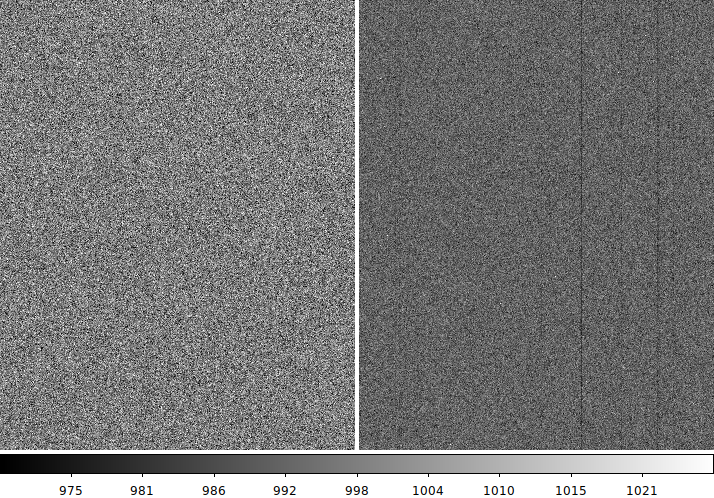
\includegraphics[width=0.8\linewidth]{pics/darkcomp.png}
    \caption{A master dark és egy nyers dark kép összehasonlítása.}
    \label{darkcomp}
\end{figure}

\subsection{Master flat}

A következő lépés a master flat elkészítése. A flat fájlokat szaturáció, gain,
bias és dark korrigáljuk átlagolás előtt.

{\bf Feladat:}
Az előző pontok és az eddigi tudásunk alapján készítsük el a master flat fájlt.
Normál esetben minden méréshez használt szűrőhöz külön master flat-et kell
készíteni. Jelen esetben csak R szűrős képek állnak a rendelkezésünkre, így elég
ehhez elkészíteni a megfelelő fájlt.

{\bf Segítség}:
Figyeljünk arra, hogy a megfelelő expozíciós idejű dark fájlt használjuk a
korrekcióhoz! Ennek a dark korrekciónak a kapcsolója az \verb+--input-master-dark+.

Szükség lesz még a \verb+--post-scale 20000+ extra kapcsolóra a ficalib parancsban.
Ezzel azonos szintre normáljuk az összes flat képünket. Erre főleg sky flatek
esetén van szükség, ahol az egyes flat képek intenzitása jelentősen eltérhet,
és ha nem skálázzuk össze a felvételeket, akkor az esetlegesen látszó csillagokat
vagy csillag csíkokat nem szedi ki jól a medián átlag.

Ha elkészültek a szaturáció, gain, bias és dark korrigált flat képeink, aklor a
következő paranccsal hozzuk létre a végső fájlt:

\begin{verbatim}
  ficombine $rflatlist --mode median -o master/flatR.fits
\end{verbatim}

{\bf Feladat:}
Nyissuk meg a master flat fájlunkat a ds9-ben. Hasonlítsuk össze egy nyers flat
fájllal. Írjuk le a tapasztalatainkat a jegyzőkönyvbe.


\subsection{Az objektumképek feldolgozása}

Amikor kész vagyunk az összes szükséges kalibrációs kép létrehozásával, akkor
korrigálhatjuk az objektum képeinket is. A sztenderd lépéseken kívül még le
fogjuk vágni a képek szélét (trimmelés), ugyanis nincs szükségünk jelen esetben
ekkora látómezőre és így helyet és számolási kapacitást spórolhatunk a
későbbiekben.

{\bf Feladat:}
Hozzuk létre az objektumfájlok nevét tartalmazó bash változót. Figyeljünk rá,
hogy a fájlok a korábban létrehozott reduced mappába kerüljenek.

A kalibrációt a következő paranccsal tudjuk végrehajtani:

\begin{verbatim}
  for FILE in $objectlist;do
      echo $FILE "feldolgozása."
      ficalib -i $FILE --input-master-bias master/BIAS.fits \
        --input-master-dark  master/mdark30.fits \
        --input-master-flat master/flatR.fits \
        --saturation 46000 --gain 1.7 -o /tmp/$FILE
      ficalib -i /tmp/$FILE --image 1400:1400:2650:2650 \
        --trim -o reduced/$FILE
      rm /tmp/$FILE
  done
\end{verbatim}

Mi történik? A ficalib elvégzi a bias, dark, flat és a szaturáció, valamint a
gain korrekciót. Ennek kimenetét egy ideiglenes fájlba mentjük, majd egy újabb
ficalib parancs elvégzi a szükséges trimmelést. Itt az \verb+--image+ kapcsolóval a
megmaradó rész pixelkoordinátáit adjuk meg x1:x2:y1:y2 formában, a \verb+--trim+ pedig
levágja az  ezen kívül eső részeket.

{\bf Feladat:}
Mikor lefutott az összes objektumképre a redukálás, nyissunk meg egyet és
hasonlítsuk össze ez nyers objektumképpel. Írjuk le a tapasztalatainkat és
készítsünk ábrát a jegyzőkönyvbe.

\section{Az objektumképek regisztrációja}

{\bf Feladat:}
Nyissuk meg az első és az utolsó kiredukált képet egy-egy külön frame-ben a ds9
segítségével. Blinkeljük össze őket (TAB billentyű). Mit tapasztalunk? Írjuk le
a jegyzőkönyvbe.

A labor végső célja, hogy a felvételeken látható pulzáló változó fénygörbéjét
elkészítsük. Ehhez meg kell mérnünk a csillag fényességét és más, úgynevezett
összehasonlító csillagok fényességét. A helyzetünket nehezíti, hogy jelen
esetben ezek a csillagok minden egyes képen más x,y pixelkoordinátákon
helyezkednek el.

Ahhoz, hogy ezt kiküszöböljük, most egy referencia képhez képest össze fogjuk
tolni a képeket, hogy mindegyik képen (hibán belül) ugyan ott legyenek a
csillagaink. Ehhez a továbbiakban bash szkripteket fogunk használni, amiket a
FITSH oldalán található példák közül fogunk kölcsönvenni.

\subsection{Csillagkeresés}

Ahhoz, hogy össze tudjuk tolni a képeket, először meg kell találnunk a képeken a
csillagokat. Ezt a fistar task segítségével fogjuk megtenni.

Látogassunk el a következő oldalra:
\url{https://fitsh.net/wiki/Example:A_composite_image_of_the_M74_galaxy}

A kedvenc text editorunkkal (nano, pico, vi, gedit, pluma, etc.) hozzunk létre
egy üres fájlt \verb+stars.sh+ néven a munkakönyvtárunkban, majd másoljuk bele az első
kódot a Registration részből.

Írjuk bele a következőket:
\begin{verbatim}
  mkdir -p astrom
  cd reduced
  ls *.fits | sed s/.fits//g > ../base.list
  cd ..
\end{verbatim}

Itt egy újabb linuxos paranccsal ismerkedünk meg, a sed-del. Ez egy nagyon
sokrétű program, mi most az egyik alapfunkcióját fogjuk felhasználni, azaz a
bemenő sorokban egy adott string-et kicserélünk egy másikra. Jelen esetben a
.fits végződést cseréljük ki a semmire, mivel a szkript kiterjesztés nélkül
várja tőlünk a bemeneteti neveket.

Írjuk át a következőket:
\begin{verbatim}
  FITS=./reduced
  SHF=1
  --flux-threshold 10000
\end{verbatim}

Mit tesz ez a fájl? Létrehoz egy új könyvtárat, astrom néven, majd létrehozza a
bemeneti listafájlt. Ezek után ez a bemenet egy while ciklusba kerül be, ami
minden egyes elemen végigmegy. A cikluson belül a fistar megekeresi nekünk a
bemeneti képen a csillagokat, majd ez kiírásra kerül egy megfelelően formázott
fájlba az astrom mappában.
A --flux-threshold kapcsolóval azt tudjuk állítani, hogy milyen halvány
forrásokat keressen a program. Minél kisebbre  állítjuk, annál halványabb
csillagokat talál meg. A jelenlegi 10000-es értékkel kb. 100 csillagot fog
megtalálni minden képen.

Mentsük el a fájlt, majd tegyük futtathatóvá. Futassuk le:

\begin{verbatim}
  ./stars.sh
\end{verbatim}

{\bf Feladat:}
Amint lefutott a szkript, nyissuk meg az első fits fájlt a reduced mappából,
majd az astrom mappába lépve nézzük meg a \verb+XX\_Cyg-20181012\_0001\_R.stars+ fájl
tartalmát. Ebben a fájlban láthatjuk a megtalált csillagok azonosítóját (első
oszlop), az x,y pixelkoordinátáit (második és harmadik oszlop), valamint
egyéb paramétereket.

A megtalált csillagokat a \verb+tvmark+ szkript segítségével plottoljuk fel:

\begin{verbatim}
  tvmark -x 2,3 -l 1 XX_Cyg-20181012_0001_R.stars
\end{verbatim}

\begin{figure}
    \centering
    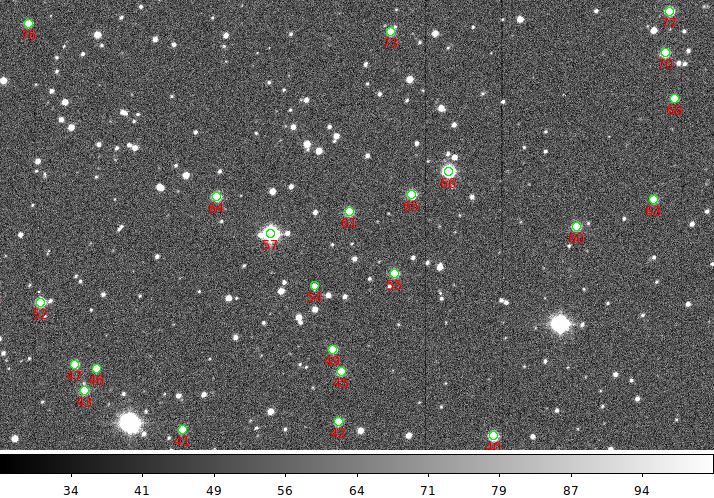
\includegraphics[width=0.8\linewidth]{pics/tvmark.png}
    \caption{A megtalált csillagok.}
    \label{stars}
\end{figure}

A \verb+-x+ kapcsolóval azt mondjuk meg, hogy a bemenő adatfájlban melyik két oszlop
az x,y koordináta, a \verb+-l+ kapcsolóval pedig, hogy melyik oszlop tartalmazza a
csillagok neveit.

Ellenőrizzük szemmel, hogy jó helyen vannak-e a felrajzolt körök és hogy
nagyságrendileg tényleg megtalált-e kb. 100 csillagot a képen a fistar.

{\bf Opcionális feladat:}
Játsszunk kicsit a treshold értékével! Próbáljuk ki kisebb, illetve nagyobb
számokkal. Plottoljuk fel a megtalált csillagokat. Mik a tapasztalatok?
Tipp: a \verb+tvmark -d+ parancs letörli a jelöléseket.

\subsection{Képtranszformációk kiszámítása}

A képek összetolásához ki kell számolnunk a megfelelő transzformációs
paramétereket. Ezeket a megtalált csillagok pozícióinak segítségével fogjuk
megtenni. A következő szkript, amit használni fogunk, minden képre kiszámolja
ezt nekünk, egy referencia képhez képest, ami most az első kép lesz.

Hozzunk létre egy új szöveges fájlt \verb+match.sh+ néven, másoljuk bele a következő kódrészletet a FITSH oldaláról.

Írjuk át a referencia fájl nevét. Vigyázzunk, hogy itt sem kell kiterjesztés!
Tegyük futtathatóvá a fájlt és futassuk is le.

\subsection{A képek összetolása}

Hozzunk létre egy új szöveges fájlt \verb+reg.sh+ néven. Másoljuk bele a következő kódrészletet.

Írjuk bele a következő sort:
\begin{verbatim}
  mkdir -p reg
\end{verbatim}

És módosítsuk a következőt:

\begin{verbatim}
  FITS=./reduced
\end{verbatim}

Tegyük futtathatóvá a fájlt és futassuk le.

{\bf Feladat:}
Nyissuk meg pár összetolt képet a ds9-ben, különböző framekben. Hasonlítsuk
őket össze. Sikerült az összetolás? Zoomoljunk ki (Zoom to fit) és blinkeljük
úgy is össze. Mit látunk? Írjuk bele tapasztalatainkat a jegyzőkönyvbe.
Készítsünk képeket a jegyzőkönyvbe az összetolt képek összehasonlításáról.

\section{Fotometria}

A végső lépés következik, azaz a fényességmérés és a fénygörbe előállítása.
Ehhez meg kell mérnünk a változó fényességét minden képen, valamint jó pár
összehasonlító csillagét is. Ezen csillagokról feltételezzük, hogy az ő
fényességük nem változott a mérés ideje alatt.

\subsection{Az XX Cyg azonosítása}

Eddig nem foglalkoztunk azzal a kérdéssel, hogy hol van pontosan a változónk a
felvételeken. Jóhiszeműen feltételeztük, hogy a felvételek jók és a csillag
valahol a képek közepe felé található. Ahhoz, hogy meg tudjuk mérni a célpont
fényességét egyértelműen azonosítanunk kell.

Keressük fel a következő oldalt:
\url{http://simbad.u-strasbg.fr/simbad/} A "Queries" ablakban kattintsunk a
"Basic search"-re. Írjuk be: XX Cyg

\begin{figure*}[!ht]
    \centering
    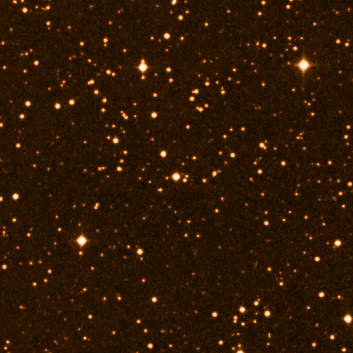
\includegraphics[width=0.6\linewidth]{pics/dss.png}
    \caption{Az ESO DSS-ben az XX Cyg környezete.}
    \label{dss}
\end{figure*}

Ha entert nyomunk, a Simbad adatbázisban a keresett csillag oldalára jutunk.
Itt számtalan informácót találunk, többek között az égi koordinátáit, a
körülbelüli fényességét különböző szűrőkben és az egyéb azonosítóit.

Mivel a mi képeink nincsenek betranszformálva csillagászati koordináta
rendszerbe (WCS, azaz World Coordinate System), kénytelenek leszünk szemmel
megkeresni.
Az első lehetőség, hogy az oldal jobb oldalán az "Interactive AladinLite view"
ablakban megnézzük, hogy hogyan néz ki a célpont környezete, majd a ds9-ben
megnyitva egy képet megpróbáljuk megtalálni. Az AladinLite ablakocskában a
görgővel lehet ki-be zoomolni.
Tipp: Technikai okokból a Schmidt kamerája, amivel ezek a felvételek készültek,
nem irányhelyesen mutatja az eget. Hogy úgy lássuk, menjünk a ds9-ben a Zoom
menübe, majd kattintsuk be az {\it Invert XY} részt és a {\it 90 degrees} részt.
Így már irányhelyesen fogjuk látni a felvételt.

Másik lehetőség, hogy elmegyünk a \url{https://archive.eso.org/dss/dss} oldalra.
Kimásoljuk a Simbad olalról a csillag ICRS koordinátáit, majd az első három
számot (hh mm ss) bemásoljuk a R.A. boxba, a második hármat pedig a Dec. boxba.
Az Image Size sorba beírunk 10-10-et, alul a legördülő menüben pedig beállítjuk,
hogy Display as GIF file.


Ha megvan a csillag, akkor tvmark-kal plottoljuk fel az első képünkön megtalált
csillagokat és jegyezzül fel a célpont sorszámát.

Ezek után válasszunk még 6 összehasonlító csillagot.
A jó összehasonlító:
\begin{itemize}
  \item Nincs túl távol a célponttól.
  \item Nem szaturált.
  \item Magányos, azaz a közvetlen közelében nincsenek más csillagok.
  \item A fényessége nagyságrendileg hasonló, mint a változóé.
\end{itemize}

Jegyezzük fel a hat összehasonlítónk sorszámát.

Ezek után hozzunk létre egy fájlt a kiválasztott csillagok neveivel és
pixelkoordinátáival. A koordinátákat az első képhez tartozó .stars fájlból
vegyük. Formátum:

\begin{verbatim}
  XX_Cyg px0 py0
  Comp1  px1 py1
  Comp2  px2 py2
  Comp3  px3 py3
  Comp4  px4 py4
  Comp5  px5 py5
  Comp6  px6 py6
\end{verbatim}

Mentsük el a fájlt \verb+phot.list+ néven. Plottoljuk fel a kiválasztott csillagokat
és készítsünk egy képet a jegyzőkönyvbe. A phot.list tartalmát táblázatként
szintén rakjuk bele a jegyzőkönyvbe.

\subsection{Apertúra fotometria}


\begin{figure*}[ht!]
    \centering
    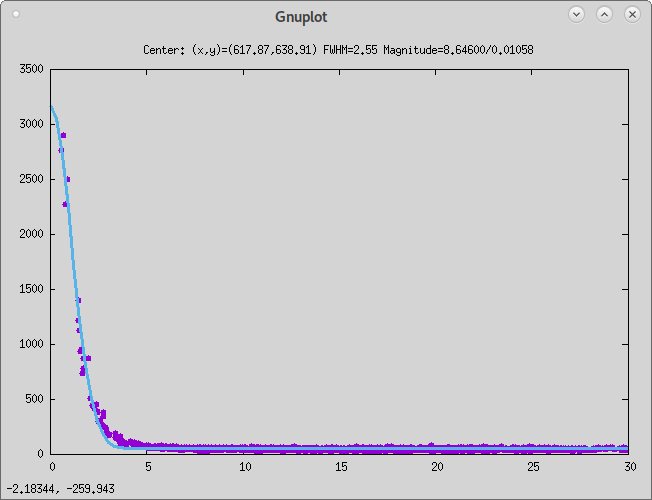
\includegraphics[width=0.7\linewidth]{pics/radialprofil.png}
    \caption{Radiális profil imexam-mal.}
    \label{radialp}
\end{figure*}

Az apertúra fotometria lényege, hogy lerakunk a képre egy a csillagra centrált
aprtúrát (kört) és azon belül megmérjük a fluxust. Ezután lerakunk a csillag
köré egy gyűrűt, amiben megmérjük az égi hátteret és ezt levonjuk a csillagon
mért fluxusból, a csillag területére arányosítva.
Ez a módszer jól működik nem túl zsúfolt csillagmezőkön, illetve akkor is, ha
valamiért a csillagok profilja nem tökéletes, vagy a távcső defókuszált.

\begin{figure}[ht!]
    \centering
    \begin{minipage}{0.45\textwidth}
        \centering
        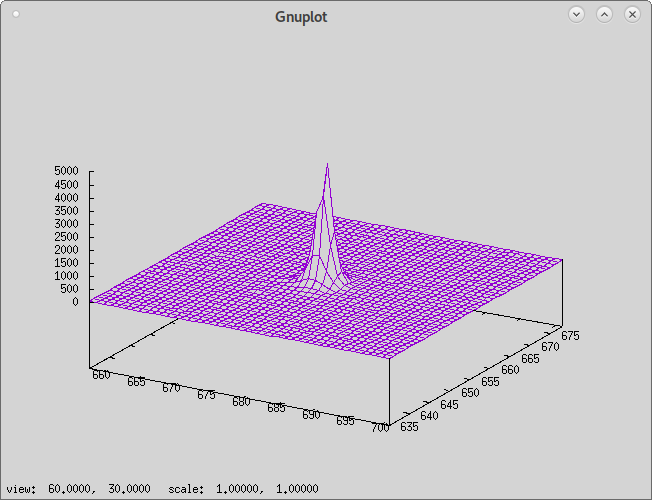
\includegraphics[width=0.9\textwidth]{pics/surface.png} % first figure itself
        \caption{Felületi plot.}
        \label{surfaceplot}
    \end{minipage}\hfill
    \begin{minipage}{0.45\textwidth}
        \centering
        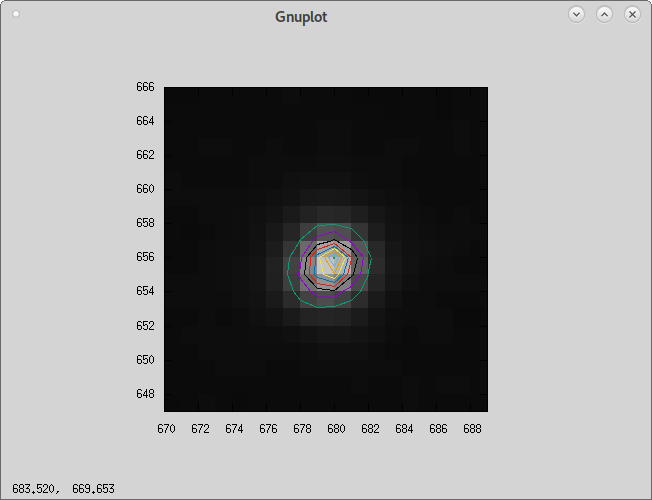
\includegraphics[width=0.9\textwidth]{pics/area.png} % second figure itself
        \caption{Kontúr plot}
        \label{areap}
    \end{minipage}
\end{figure}

Hátránya, hogy sűrű területeken az egymásba lógó és sűrűn elhelyezkedő
csillagok miatt nem ad jó eredményt. Ebben az esetben PSF fotometriát kell
alkalmazni, ami a csillagprofilokat illeszti meg és az alapján számol fluxust.
Mi ez utóbbi módszert relatíve bonyolult természete miatt nem fogjuk használni,
valamint azért sem, mert a mi esetünkben a csillagaink kellően távol
helyezkednek el egymástól.

A megfelelő aprtúra és égi gyűrű kiválasztása soha sem egyszerű feladat. Támpont
lehet a csillagprofilok félértékszélessége (FWHM). Csillagaink egy Moffat
függvénnyel (vagy egy Gauss-os alakkal) jól közelíthető profillal rendelkeznek.
Vizsgáljuk meg őket közelebbről!

{\bf Feladat:}
Nyissunk meg egy összetolt képet ds9-ben. Indítsuk el az imexam taskot.
Ha a ds9-re visszük a kurzort láthatjuk, hogy megváltozott. Keressünk egy
kellően fényes csillagot, vigyük a közepére a kurzort, majd nyomjuk meg az
{\it r} gombot. Ekkor a csillagprofil radiális plotját láthatjuk. Az {\it s}
betűt lenyomva egy felületi plotot látunk, az {\it e} betűvel pedig egy kontúr
plotot láthatunk.

A radiális plot esetén felül látunk egy becsült félértékszélesség értéket.
Ezt mérjük meg 10 csillagra, majd átlagoljuk és jegyezzük fel ezt a számot.
Vigyázzunk, hogy a csillagok ne legyenek szaturáltak és hogy magányosak
legyenek.


Hogy ki tudjuk választani a megfelelő apertúrát, több különböző értékre is
lefuttatjuk a fotometriát. Szerencsére a FITSH fiphot csomagja ezt kényelmes
módon támogatja.

Hozzunk létre egy új fált phot.sh néven és másoljuk bele a következőt:

\begin{verbatim}
mkdir -p phot
FITS=./reg
PHOT=./phot

cat base.list | \
  while read base dummy ; do
      fiphot $FITS/$base.fits --input-list phot.list --col-id 1 --col-xy 2,3 \
                              --apertures ... \
                              --sky-fit median \
                              --format IXY,MmFfBbs \
                              --comment --output $PHOT/$base.phot
  done
\end{verbatim}

\begin{figure*}[ht!]
    \centering
    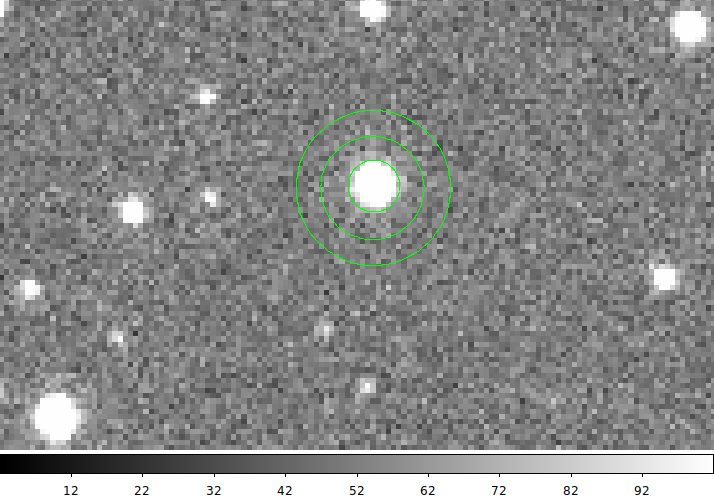
\includegraphics[width=0.6\linewidth]{pics/aperture.png}
    \caption{Példa apertúra és égi gyűrű egy csillag körül.}
    \label{apert}
\end{figure*}

Ahol az apertures ... részt helyettesítsük a következő módon:
A kiszámolt átlagos félértékszélességet kerekítsük fel egészre, majd egyesével
növeljük az értékét öt lépésen keresztül. Így lesz 6 számunk, ami az apertúra
sugarát adja meg. Ezek után nézzük meg a legnagyobb számot és az égi gyűrű belső
sugarának válasszunk egy ennél pár pixellel nagyobb számot. A külső sugárnak
pedig egy ennél kb. nyolccal nagyobb számot.

Azaz, ha pl. az átlag félértékszélességünk 3.78, akkor az első szám 4, majd 5,
6, 7, 8, 9, az apertúra belső sugara 12, a külső pedig 20.
Ezeket a következő formában kell a fiphot-nak megadni a \verb+--apertures+ kapcsoló után: \verb+4:12:20,5:12:20,6:12:20,7:12:20,8:12:20,9:12:20+
Figyelem, az itt bemutatott értékek nem biztos, hogy a jó apertúra értékek!

Figyeljük meg, hogy az égi gyűrű mérete mindegyik apertúrához ugyanakkora!

Futassuk le a \verb+phot.sh+-t és nézzük meg a keletkezett fájlokat a phot mappában.
Milyen a fájlok szerkezete? Tipp: nézzük meg a szkriptben a \verb+fiphot+ parancs
\verb+--format+ kapcsolója után megadott formátumot.


{\bf Extra opcionális feladat:}
Ha nagyon pontos fotometriát akarunk, akkor az összetolt képeken érdemes
újracentrálni (azaz megkeresni a közepét) a fotometrálandó csillagainknak,
ugyanis a képek regisztrációja nem 100\%-ig pontos, tehát a gyakorlatban egy
nagyon picit minden csillag máshol van, mint a referencia képen. A mi
esetünkben ez most nem gond, de általában érdmes ezt megtenni.
Ha valaki érez magában erőt, akkor írjon egy szkriptet, ami minden összetolt
képen újracentrálja a mérendő csillagokat és ezeket a centrált pixel
kooordinátákat használja majd fel az aktuális fotometriához. Ha valaki így
tesz, akkor ehhez a fenti szkriptet is módosítania kell.


{\bf Feladat:}
Ellenőrizzük le az apertúrákat.
Az első fájlhoz tartozó phot fájlból szedjük ki a célponthoz tartozó
magnitúdó értékeket. Írjuk bele egy fájlba úgy, hogy az első oszlopba az adott
apertúra sugarának az értéke kerüljön, a másodikba pedig a fényesség
magnitúdóban.

Mentsük el a fájlt cog.dat néven, majd indítsunk egy gnuplotot. Az úgynevezett
növekedési görbét fogjuk elkészíteni, ami azt mutatja meg, hogy az apertúra
változásával hogyan változik egy adott forrás fényessége.

A gnuplotban adjuk ki a következő parancsokat:
\begin{verbatim}
  set yrange [] rev
  unset key
  plot 'cog.dat'
\end{verbatim}

Vizsgáljuk meg az elkészült ábrát. Mit látunk? Miért kellett megfordítani az y
tengelyt? Milyen következtetést tudunk levonni az apertúrák nagyságáról a
fotometria szempontjából? Az ábrát rakjuk be a jegyzőkönyvbe és írjuk le a
tapasztalatainkat is.

Ha kell, akkor írjuk át az apertúrák méretét és futassuk le újra a phot.sh-t.
Készítsük el újra a növekedési görbét.

Válasszuk ki azt az apetrúrát, amivel a továbbiakban dolgozni akarunk.
Hogy haladni tudjunk, ki kell szednünk a kiválasztott apertúránkhoz tartozó
magnitúdó értékeket a fotometriai adatfájlokból.
Kicsit előre kell most gondolkodnunk. A végső fénygörbe plot úgy fog előállni,
hogy az idő függvényében ábrázoljuk a célpont fényességének változását egy
összehasonlító fényességéhez képest. Ezt az ábrát majd a gnuplottal fogjuk
létrehozni. A gnuplotnak jól struktúrált bemenetre van szüksége, ahol az egyes
pontokat az egyes sorok alapján fogja ábrázolni.

Ezért a következő adatszerkezetre van szükségünk a végső adatfájlban:
\begin{verbatim}
  idő változó_mag változó_mag_err comp1_mag comp1_err comp2_mag comp2_err ....
\end{verbatim}

Ahol a magnitúdóban lévő fényességek az általunk kiválasztott apertúrával mért
fényességek lesznek.
Az időt a fits fájlok fejlécéből tudjuk kinyerni. Az egyszerű plottolhatóság
kedvéért Julián dátumban. A Julián dátum a Kr. e. 4713. január elseje, UTC 12
óra óta eltelt napok száma. Ez szerencsére benne van a fejlécekben a JD
kulcsszóban.

{\bf Feladat:}
Próbáljuk meg magunktól létrehozni a végső adatfájlt a fent látott formátumban.

\subsection{Differenciális fotometria}

A következőkben a csillagunk fénygörbéjét fogjuk előállítani. Hogy kinek melyik
összehasonlító lesz jó a végén, az nagyban függ az egyénileg kiválasztott
csillagoktól.

{\bf Feladat:}
Először plottoljuk fel a változó fényességét az első összehasonlítóhoz képest a
gnuplotban.

\begin{verbatim}
  set yrange [] rev
  plot 'XX_Cyg.data' u ($1-2450000):($2-$4)
\end{verbatim}
A Julián dátumból a kényelmesebb leolvashatóság kedvéért vontuk le a 2450000-t.

Mit látunk? Próbáljuk meg a többi összehasonlítóval is ábrázolni a
differenciális fénygörbét.

Ha megvan a szerintünk legjobbnak gondolt összehasonlító, akkor el kell
végeznünk egy tesztet, hogy a csillag nem változó-e. Mivel csak szemre
választottunk csillagokat és nem ellenőriztük csillagkatalógusból a forrásokat,
ezért ebben nem lehetünk biztosak.

{\bf Feladat:}
Plottoljuk fel a kedvenc összehasonlítónkat a többi összehasonlítóhoz képest.
Mit látunk? Változik-e az összehasonlító? Ha igen, akkor keressünk egy olyat,
amelyik nem. Ezt is ellenőrizzük le több másik összehasonlítóval.

\begin{figure*}[ht!]
    \centering
    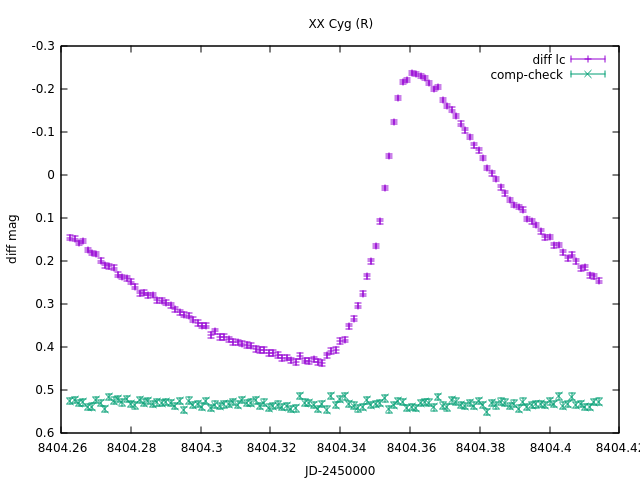
\includegraphics[width=0.65\linewidth]{pics/lc.png}
    \caption{Az XX Cyg fénygörbéje és a comp-check.}
    \label{lc}
\end{figure*}

Ha megvan a legjobb összehasonlító, ami nem változó, akkor készítsük el a
végső plotot. Adjunk címet az ábrának, feliratozzuk a tengelyeket, a
jelmagyarázatba írjunk értelmes szöveget és a változónk fénygörbéje alá
plottoljuk fel az úgynevezett comp-check-et is, azaz a használt összehasonlító
fényessége mínusz egy másik összehasonlító. Plottoljuk fel a hibákat is!
Az ábrát rakjuk bele a jegyzőkönyvbe.
Segítség:
\url{http://lowrank.net/gnuplot/plot2-e.html}

Becsüljük meg a csillag peak-to-peak amplitúdóját. Becsüljünk hibát is.
Írjuk bele a jegyzőkönyvbe az eredményt.

\section{Jegyzőkönyv}

A jegyzőkönyvet a labor alatt elvégzett munkáról kell megírni, pár oldal
terjedelemben. Mindenkitől külön jegyzőkönyvet várunk. A jegyzőkönyv várt
formátuma pdf. A végső jegyzőkönyvet a labor után maximum 1-2 héttel kell
elküldeni a laborvezetőknek értékelésre.

\end{document}
